\documentclass[14pt]{extbook}
\usepackage{multicol, enumerate, enumitem, hyperref, color, soul, setspace, parskip, fancyhdr} %General Packages
\usepackage{amssymb, amsthm, amsmath, latexsym, units, mathtools} %Math Packages
\everymath{\displaystyle} %All math in Display Style
% Packages with additional options
\usepackage[headsep=0.5cm,headheight=12pt, left=1 in,right= 1 in,top= 1 in,bottom= 1 in]{geometry}
\usepackage[usenames,dvipsnames]{xcolor}
\usepackage{dashrule}  % Package to use the command below to create lines between items
\newcommand{\litem}[1]{\item#1\hspace*{-1cm}\rule{\textwidth}{0.4pt}}
\pagestyle{fancy}
\lhead{Progress Quiz 10}
\chead{}
\rhead{Version B}
\lfoot{5170-5105}
\cfoot{}
\rfoot{Summer C 2021}
\begin{document}

\begin{enumerate}
\litem{
Choose the graph of the equation below.\[ f(x) = \sqrt[3]{x - 10} - 4 \]\begin{enumerate}[label=\Alph*.]
\begin{multicols}{2}\item 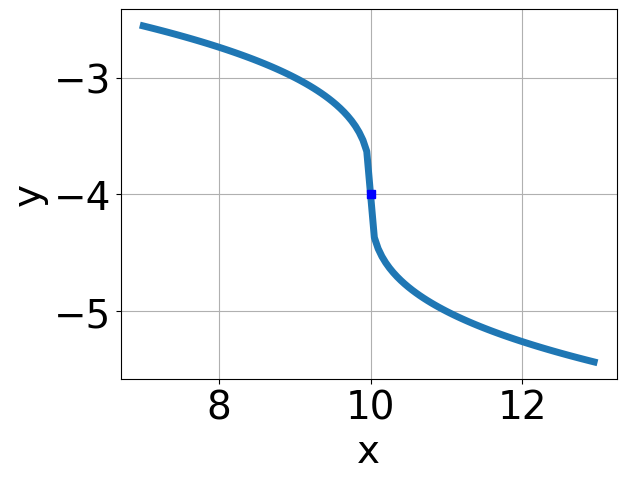
\includegraphics[width = 0.3\textwidth]{../Figures/radicalEquationToGraphAB.png}\item 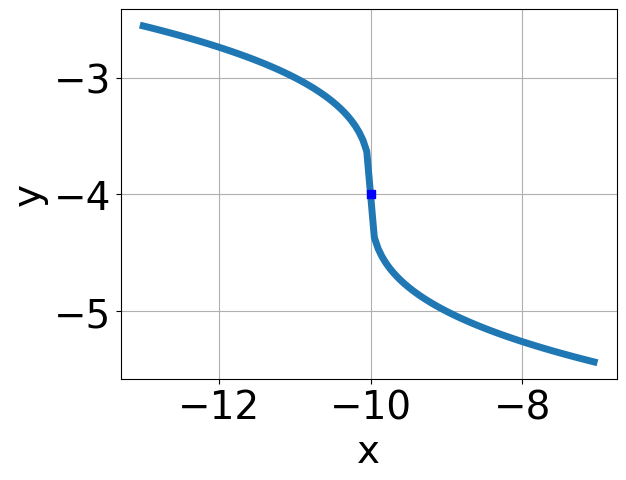
\includegraphics[width = 0.3\textwidth]{../Figures/radicalEquationToGraphBB.png}\item 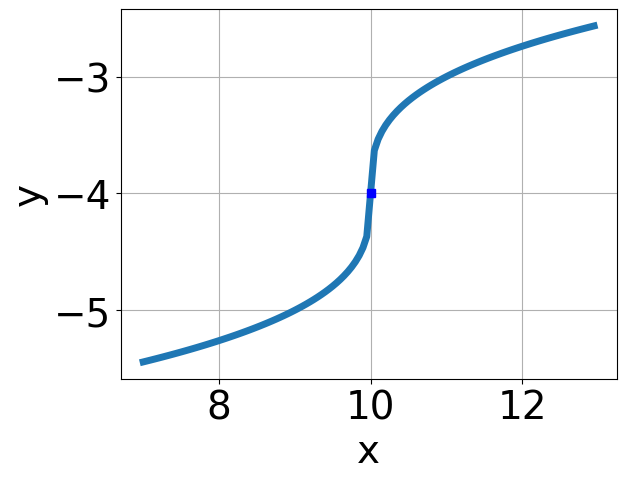
\includegraphics[width = 0.3\textwidth]{../Figures/radicalEquationToGraphCB.png}\item 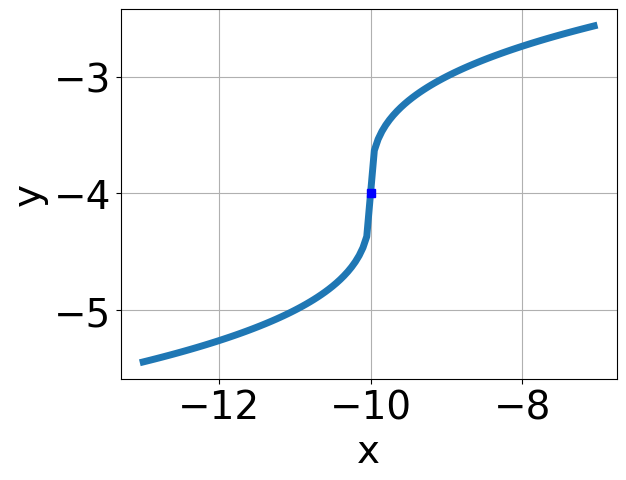
\includegraphics[width = 0.3\textwidth]{../Figures/radicalEquationToGraphDB.png}\end{multicols}\item None of the above.
\end{enumerate} }
\litem{
Solve the radical equation below. Then, choose the interval(s) that the solution(s) belongs to.\[ \sqrt{-56 x^2 + 12} - \sqrt{-26 x} = 0 \]\begin{enumerate}[label=\Alph*.]
\item \( x \in [0.48,0.99] \)
\item \( x_1 \in [-0.12, 0.53] \text{ and } x_2 \in [-0.25,4.75] \)
\item \( \text{All solutions lead to invalid or complex values in the equation.} \)
\item \( x_1 \in [-0.84, -0.19] \text{ and } x_2 \in [-0.25,4.75] \)
\item \( x \in [-0.84,-0.19] \)

\end{enumerate} }
\litem{
Choose the equation of the function graphed below.
\begin{center}
    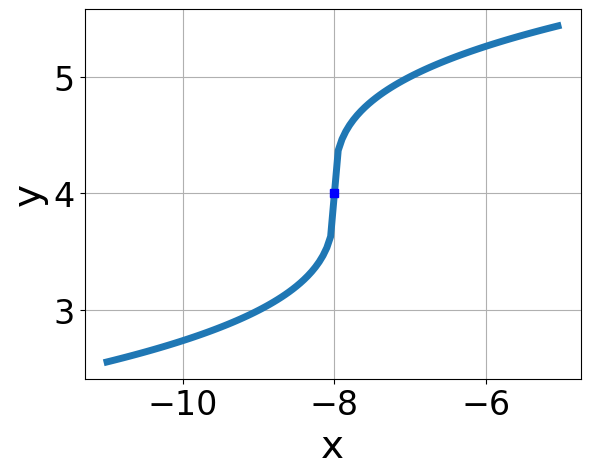
\includegraphics[width=0.5\textwidth]{../Figures/radicalGraphToEquationB.png}
\end{center}
\begin{enumerate}[label=\Alph*.]
\item \( f(x) = - \sqrt[3]{x + 8} + 4 \)
\item \( f(x) = \sqrt[3]{x - 8} + 4 \)
\item \( f(x) = - \sqrt[3]{x - 8} + 4 \)
\item \( f(x) = \sqrt[3]{x + 8} + 4 \)
\item \( \text{None of the above} \)

\end{enumerate} }
\litem{
Choose the graph of the equation below.\[ f(x) = - \sqrt{x - 6} + 3 \]\begin{enumerate}[label=\Alph*.]
\begin{multicols}{2}\item 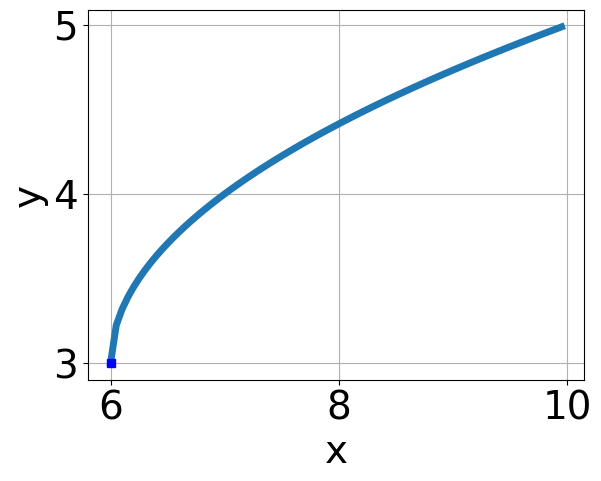
\includegraphics[width = 0.3\textwidth]{../Figures/radicalEquationToGraphCopyAB.png}\item 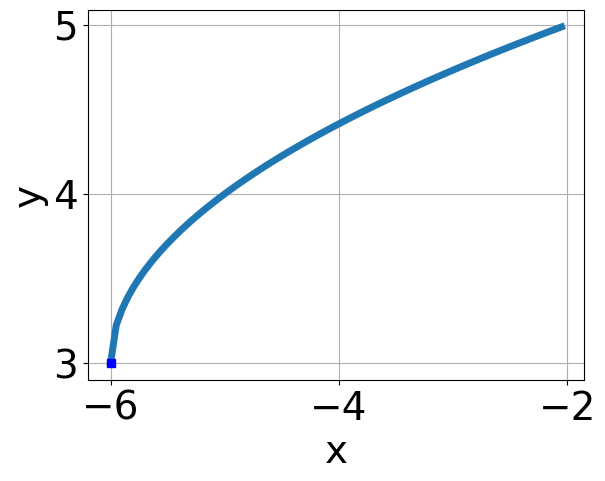
\includegraphics[width = 0.3\textwidth]{../Figures/radicalEquationToGraphCopyBB.png}\item 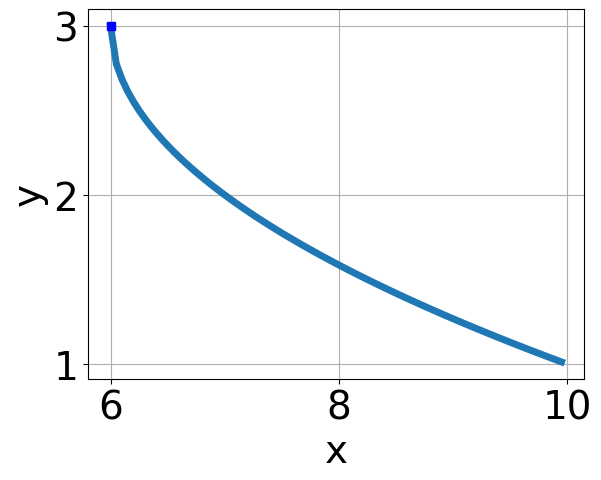
\includegraphics[width = 0.3\textwidth]{../Figures/radicalEquationToGraphCopyCB.png}\item 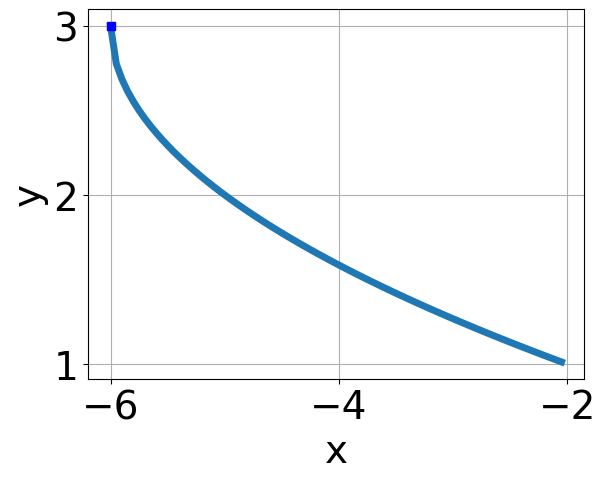
\includegraphics[width = 0.3\textwidth]{../Figures/radicalEquationToGraphCopyDB.png}\end{multicols}\item None of the above.
\end{enumerate} }
\litem{
What is the domain of the function below?\[ f(x) = \sqrt[5]{-5 x + 6} \]\begin{enumerate}[label=\Alph*.]
\item \( \text{The domain is } [a, \infty), \text{   where } a \in [1.06, 1.44] \)
\item \( \text{The domain is } [a, \infty), \text{   where } a \in [0.72, 1.05] \)
\item \( \text{The domain is } (-\infty, a], \text{   where } a \in [0.88, 1.42] \)
\item \( (-\infty, \infty) \)
\item \( \text{The domain is } (-\infty, a], \text{   where } a \in [0.58, 0.88] \)

\end{enumerate} }
\litem{
Solve the radical equation below. Then, choose the interval(s) that the solution(s) belongs to.\[ \sqrt{8 x + 6} - \sqrt{2 x - 8} = 0 \]\begin{enumerate}[label=\Alph*.]
\item \( x_1 \in [-3.04, -1.63] \text{ and } x_2 \in [-5.75,3.25] \)
\item \( x \in [0.14,0.6] \)
\item \( \text{All solutions lead to invalid or complex values in the equation.} \)
\item \( x \in [-3.04,-1.63] \)
\item \( x_1 \in [-1.66, -0.2] \text{ and } x_2 \in [2,9] \)

\end{enumerate} }
\litem{
Solve the radical equation below. Then, choose the interval(s) that the solution(s) belongs to.\[ \sqrt{8 x + 4} - \sqrt{7 x + 8} = 0 \]\begin{enumerate}[label=\Alph*.]
\item \( \text{All solutions lead to invalid or complex values in the equation.} \)
\item \( x \in [3.31,4.38] \)
\item \( x_1 \in [-1.15, -0.8] \text{ and } x_2 \in [-3.5,1.5] \)
\item \( x_1 \in [-1.05, -0.39] \text{ and } x_2 \in [2,9] \)
\item \( x \in [-12.21,-11.83] \)

\end{enumerate} }
\litem{
What is the domain of the function below?\[ f(x) = \sqrt[7]{-9 x - 3} \]\begin{enumerate}[label=\Alph*.]
\item \( (-\infty, \infty) \)
\item \( \text{The domain is } [a, \infty), \text{   where } a \in [-4, -2] \)
\item \( \text{The domain is } (-\infty, a], \text{   where } a \in [-1.7, -0.2] \)
\item \( \text{The domain is } (-\infty, a], \text{   where } a \in [-3.9, -1.9] \)
\item \( \text{The domain is } [a, \infty), \text{   where } a \in [-1.33, 0.67] \)

\end{enumerate} }
\litem{
Choose the equation of the function graphed below.
\begin{center}
    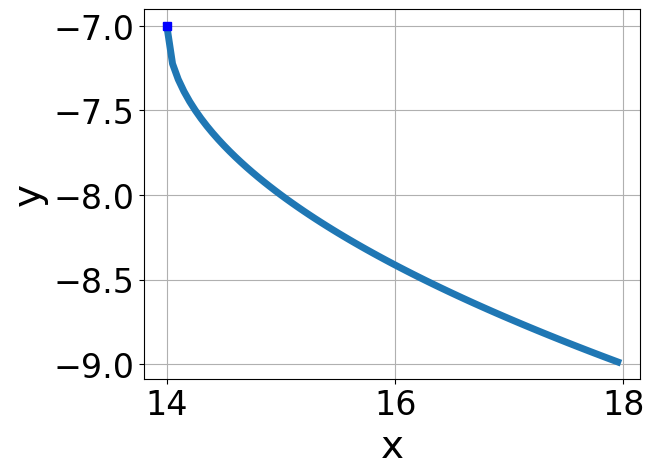
\includegraphics[width=0.5\textwidth]{../Figures/radicalGraphToEquationCopyB.png}
\end{center}
\begin{enumerate}[label=\Alph*.]
\item \( f(x) = \sqrt{x - 14} - 7 \)
\item \( f(x) = \sqrt{x + 14} - 7 \)
\item \( f(x) = - \sqrt{x - 14} - 7 \)
\item \( f(x) = - \sqrt{x + 14} - 7 \)
\item \( \text{None of the above} \)

\end{enumerate} }
\litem{
Solve the radical equation below. Then, choose the interval(s) that the solution(s) belongs to.\[ \sqrt{30 x^2 + 36} - \sqrt{-69 x} = 0 \]\begin{enumerate}[label=\Alph*.]
\item \( \text{All solutions lead to invalid or complex values in the equation.} \)
\item \( x_1 \in [-0.08, 1.88] \text{ and } x_2 \in [1.33,1.81] \)
\item \( x \in [-1.14,-0.53] \)
\item \( x_1 \in [-2.84, -1.13] \text{ and } x_2 \in [-2.44,-0.24] \)
\item \( x \in [-2.84,-1.13] \)

\end{enumerate} }
\end{enumerate}

\end{document}